\documentclass[border=4pt]{standalone}
\usepackage{amsmath,amssymb,tikz}
\usetikzlibrary{arrows.meta,calc}
\definecolor{figB}{RGB}{31,90,166}\definecolor{figR}{RGB}{176,48,48}\definecolor{figG}{RGB}{46,125,50}\definecolor{figO}{RGB}{214,120,20}
\begin{document}
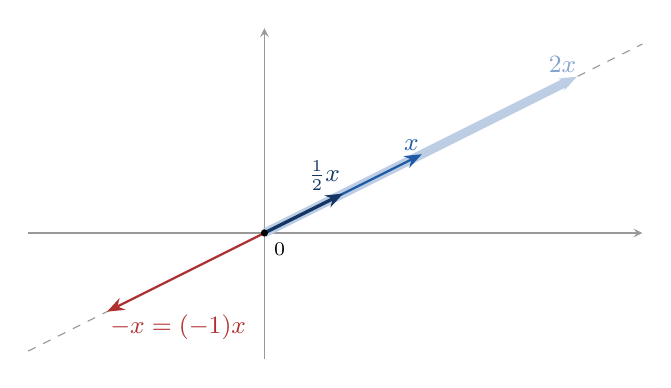
\begin{tikzpicture}[scale=1.0,>={Stealth[length=2.2mm]}]
\draw[-stealth,thin,black!40] (-3,0)--(4.8,0);
\draw[-stealth,thin,black!40] (0,-1.6)--(0,2.6);
\draw[black!40,dashed] (-3.0,-1.5)--(4.8,2.4);
\draw[->,line width=3.2pt,figB!30,shorten >=1pt] (0,0)--(4,2);
\draw[->,thick,figB] (0,0)--(2,1);
\draw[->,very thick,figB!60!black] (0,0)--(1,0.5);
\draw[->,thick,figR] (0,0)--(-2,-1);
\node[font=\small,figB,above left,inner sep=1pt] at (2,1) {$x$};
\node[font=\small,figB!55,above left,inner sep=1pt] at (4,2) {$2x$};
\node[font=\small,figB!60!black,above left,inner sep=1pt] at (1,0.5) {$\tfrac12x$};
\node[font=\small,figR,below right,inner sep=1pt] at (-2,-1) {$-x=(-1)x$};
\fill (0,0) circle (1.3pt) node[below right,font=\scriptsize]{$0$};
\end{tikzpicture}
\end{document}
